\section{Forward/Tangent-Linear Model Tests}
%===========================================
Before discussing the results of the forward/tangent-linear model tests (FWD/TL test), a short description of the test itself is warranted. The FWD/TL test is not a ``pass-or-fail'' type of test, but is performed to allow assessment of the behaviour of the forward and tangent-linear model over a range of perturbations to the model variables. The input variables (temperature, cloud particle effective radius, and cloud water content for the CloudScatter test; aerosol particule effective radius and aerosol concentration for the AersosolScatter test) are perturbed 15 times decreasing from a maximum fraction of 0.1, with each subsequent perturbation being half of the previous one. Thus the final perturbation applied is approximately $6\times 10^{-6}$.
 
 
\subsection{CloudScatter Module}
%-------------------------------
\subsubsection{Insufficient range in LUT}
%........................................
\label{sec:Insufficient.LUT.range.Cloud}
Cases arise where the input cloud properties (temperature and effective radius) fall outside the range of data covered in the cloud optical properties LUT. In the forward model case, when this happens no extrapolation is performed - the LUT extrema values are simply returned. In the tangent-linear model case, the returned result is always zero.

A comparison of test output for the water cloud case for AMSU-A ch.8 (55.5GHz) inspecting the variation of the optical depth as a function of temperature is shown in figure \ref{fig:amsua_n18.ch8.WATER.dOd_dT}. The cloud optical property LUT temperature range is (currently) 263.16-300K. The layer cross-section shown in figure \ref{fig:amsua_n18.ch8.WATER.dOd_dT} is at 695hPa which, for the tropical climatology, has a temperature of 282.14K. The $\pm$0.1 perturbation fraction for the temperature yields 253.9K (-0.1) and 310.3K (+0.1). Because these values are outside the LUT temperature range, the forward model simply returns the 263.16 and 300K values for the -0.1 and +0.1 temperature perturbation respectively and that leads to the ``kinks'' in the non-linear response of figure \ref{fig:amsua_n18.ch8.WATER.dOd_dT}. Note that the feature occurs irrespective of the interpolation method. The tangent-linear result is not impacted in this particular case because the tangent-linear optical depth is not directly affected by the temperature perturbation, but only by the dependence of the mass extinction coefficient on the temperature perturbation - which, for temperatures outside the LUT range, is zero.

\begin{figure}[htp]
  \centering
  \begin{tabular}{c c c}
    \multicolumn{3}{c}{\qquad\sffamily\textbf{NOAA-18 AMSU-A ch.8}}\\
    \multicolumn{3}{c}{\qquad\sffamily\textbf{Water cloud test case}}\\
    \qquad\textsf{(a)} & \qquad\textsf{(b)}  & \qquad\textsf{(c)} \\
    \qquad\textsf{Linear} & \qquad\textsf{Cubic}  & \qquad\textsf{Averaged Quadratic} \\
    \includegraphics[bb=90 400 300 540,clip,scale=0.7]{graphics/Cloud/TL/amsua_n18.ch8.WATER.NLIN.dOd_dT.eps} &
    \includegraphics[bb=90 400 300 540,clip,scale=0.7]{graphics/Cloud/TL/amsua_n18.ch8.WATER.NCUBIC.dOd_dT.eps}  &
    \includegraphics[bb=90 400 300 540,clip,scale=0.7]{graphics/Cloud/TL/amsua_n18.ch8.WATER.AVGQUAD.dOd_dT.eps}
  \end{tabular}
  \caption{Effect of insufficient range in the cloud optical property LUT. Comparison of forward, non-linear (red) and tangent-linear (black) model optical depth variation with respect to temperature at 695hPa for the NOAA-18 AMSU-A ch.8 water cloud case using \textbf{(a)} linear, \textbf{(b)} cubic, and \textbf{(c)} averaged quadratic interpolation. The deviations in the non-linear response for the larger perturbations is due to the input cloud temperature data extending beyond that defined in the LUT. Symbol positions indicate the perturbation fractions at which the calculations were performed.}
  \label{fig:amsua_n18.ch8.WATER.dOd_dT}
\end{figure}

\subsubsection{Discontinuous Derivatives}
%........................................
\label{sec:Discontinuous.derivatives.Cloud}
The biggest problem for the simpler polynomial interpolation schemes being tested here is the fact that the interpolating function derivatives are discontinuous across LUT hingepoints. The effects of this appear as regular failures of linear interpolation and occasional failures of cubic interpolation. The following documents the character of this failures.

A comparison of test output for the snow cloud case for AMSU-A ch.8 (55.5GHz) inspecting the variation of the optical depth as a function of effective radius at 400hPa is shown in figure \ref{fig:amsua_n18.ch8.SNOW.dOd_dReff.TL}. Here, linear interpolation clearly highlights the derivative discontinuity when crossing over hinge-points in the LUT data. Inspection of the LUT dimension vectors lists the effective radii for the microwave cases as [10, 50, 250, 500, 750, 1000] and the test profile parameters for the snow cloud case shown in table \ref{tab:Test.Profile.cloud_parameters} indicate the maximum effective radius is 500\micron. Thus, as the forward model effective radius is perturbed beyond 500\micron, any subsequent linear interpolation of the LUT data will yield discontinuous derivatives. The linear case, figure \ref{fig:amsua_n18.ch8.SNOW.dOd_dReff.TL}(a), shows this most clearly: as soon as the effective radius changes from $<$500\micron{} to $>$500\micron, there is an abrupt change in the slope of the forward, non-linear result. This effect is not apparent in the corresponding plot for the cubic interpolation case but, as is shown later, that is due to a combination of the scale of the plot (i.e. the discontinuity is there, just not visible) and serendipity (i.e. it just so happens that the derivatives of the interpolating polynomials are nearly equal across the LUT hingepoint). The result using averaged quadratic interpolation, figure \ref{fig:amsua_n18.ch8.SNOW.dOd_dReff.TL}(c), appears similar to that for cubic interpolation, but with slightly different response curve slopes.

\begin{figure}[htp]
  \centering
  \begin{tabular}{c c c}
    \multicolumn{3}{c}{\qquad\sffamily\textbf{NOAA-18 AMSU-A ch.8}}\\
    \multicolumn{3}{c}{\qquad\sffamily\textbf{Snow cloud test case}}\\
    \qquad\textsf{(a)} & \qquad\textsf{(b)}  & \qquad\textsf{(c)} \\
    \qquad\textsf{Linear} & \qquad\textsf{Cubic}  & \qquad\textsf{Averaged Quadratic} \\
    \includegraphics[bb=90 400 300 540,clip,scale=0.7]{graphics/Cloud/TL/amsua_n18.ch8.SNOW.NLIN.dOd_dReff.eps} &
    \includegraphics[bb=90 400 300 540,clip,scale=0.7]{graphics/Cloud/TL/amsua_n18.ch8.SNOW.NCUBIC.dOd_dReff.eps} &
    \includegraphics[bb=90 400 300 540,clip,scale=0.7]{graphics/Cloud/TL/amsua_n18.ch8.SNOW.AVGQUAD.dOd_dReff.eps} 
  \end{tabular}
  \caption{Effect of discontinuous derivatives in the FWD/TL test. Comparison of forward, non-linear (red) and tangent-linear (black) model optical depth variation with respect to particle effective radius at 400hPa for the NOAA-18 AMSU-A ch.8 snow cloud case using different interpolation schemes. See figure \ref{fig:Test.Profile4} for the snow cloud water content and effective radius profiles.  \textbf{(a)} Linear interpolation. The abrubt change in the non-linear result slope occurs as the perturbations cross a LUT hingepoint (see text for details). \textbf{(b)} Cubic interpolation of the LUT data in this case does not lead to any noticable discontinuity. \textbf{(c)} Averaged quadratic interpolation preserves the derivatives across LUT higepoints, but note the slopes are slightly different. Symbol positions indicate the perturbation fractions at which the calculations were performed.}
  \label{fig:amsua_n18.ch8.SNOW.dOd_dReff.TL}
\end{figure}

A similar result is obtained in the snow cloud case for HIRS/4 ch.8 (900\invcm), but in this case the difference between cubic and averaged quadratic interpolation is more pronounced. Figure \ref{fig:hirs4_n18.ch8.SNOW.dg_dReff.TL} shows the variation of the asymmetry parameter with respect to effective radius at the 217hPa layer pressure (near the top of the snow cloud). For the linear interpolation case, we see the characteristic abrupt change in the non-linear slope across a LUT hinge-point, whereas for the cubic interpolation case the non-linear response is better behaved. The averaged quadratic interpolation result is quite different from the cubic interpolation case, with a significantly different tangent-linear slope, and a non-linear response that is more pronounced and with opposite curvature with respect to increasing perturbations.

\begin{figure}[htp]
  \centering
  \begin{tabular}{c c c}
    \multicolumn{3}{c}{\qquad\sffamily\textbf{NOAA-18 HIRS/4 ch.8}}\\
    \multicolumn{3}{c}{\qquad\sffamily\textbf{Snow cloud test case}}\\
    \qquad\textsf{(a)} & \qquad\textsf{(b)}  & \qquad\textsf{(c)} \\
    \qquad\textsf{Linear} & \qquad\textsf{Cubic}  & \qquad\textsf{Averaged Quadratic} \\
    \includegraphics[bb=90 400 300 540,clip,scale=0.7]{graphics/Cloud/TL/hirs4_n18.ch8.SNOW.NLIN.dg_dReff.eps} &
    \includegraphics[bb=90 400 300 540,clip,scale=0.7]{graphics/Cloud/TL/hirs4_n18.ch8.SNOW.NCUBIC.dg_dReff.eps} &
    \includegraphics[bb=90 400 300 540,clip,scale=0.7]{graphics/Cloud/TL/hirs4_n18.ch8.SNOW.AVGQUAD.dg_dReff.eps} 
  \end{tabular}
  \caption{Effect of discontinuous derivatives in the FWD/TL test. Comparison of forward, non-linear (red) and tangent-linear (black) model asymmetry parameter variation with respect to particle effective radius at 217hPa for the NOAA-18 HIRS/4 ch.8 snow cloud case using different interpolation schemes. See figure \ref{fig:Test.Profile4} for the snow cloud water content and effective radius profiles. \textbf{(a)} Linear interpolation. The abrubt change in the non-linear result slope occurs as the perturbations cross a LUT hingepoint (see text for details). \textbf{(b)} Cubic interpolation of the LUT data in this case does not lead to any noticeable discontinuity. \textbf{(c)} Averaged quadratic interpolation preserves the derivatives across LUT higepoints, but note the tangent-linear slope and character of the non-linar response are quite different from the cubic interpoaltion case. Symbol positions indicate the perturbation fractions at which the calculations were performed.}
  \label{fig:hirs4_n18.ch8.SNOW.dg_dReff.TL}
\end{figure}

A comparison of test results for the rain cloud case for AMSU-A ch.15 (89GHz), inspecting the variation of the optical depth as a function of effective radius at 918hPa, is shown in figure \ref{fig:amsua_n18.ch15.RAIN.dOd_dReff}. This case is mentioned because changing the interpolation scheme yields results that differ in sign: the linear interpolation scheme produces a negative tangent-linear slope, while the cubic and averaged quadratic produce a positive slope. Similarly for the non-linear response near zero perturbation.

\begin{figure}[htp]
  \centering
  \begin{tabular}{c c c}
    \multicolumn{3}{c}{\qquad\sffamily\textbf{NOAA-18 AMSU-A ch.15}}\\
    \multicolumn{3}{c}{\qquad\sffamily\textbf{Rain cloud test case}}\\
    \qquad\textsf{(a)} & \qquad\textsf{(b)}  & \qquad\textsf{(c)} \\
    \qquad\textsf{Linear} & \qquad\textsf{Cubic}  & \qquad\textsf{Averaged Quadratic} \\
    \includegraphics[bb=90 400 300 540,clip,scale=0.7]{graphics/Cloud/TL/amsua_n18.ch15.RAIN.NLIN.dOd_dReff.eps} &
    \includegraphics[bb=90 400 300 540,clip,scale=0.7]{graphics/Cloud/TL/amsua_n18.ch15.RAIN.NCUBIC.dOd_dReff.eps} &
    \includegraphics[bb=90 400 300 540,clip,scale=0.7]{graphics/Cloud/TL/amsua_n18.ch15.RAIN.AVGQUAD.dOd_dReff.eps} 
  \end{tabular}
  \caption{Impact of interpolation scheme on response slope. Comparison of forward, non-linear (red) and tangent-linear (black) model optical depth variation with respect to particle effective radius at 918hPa for the NOAA-18 AMSU-A ch.15 rain cloud case using different interpolation schemes. See figure \ref{fig:Test.Profile3} for the rain cloud water content and effective radius profiles. \textbf{(a)} Linear interpolation. Tangent-linear response, and non-linear response as $\delta x \rightarrow\pm 0$, have negative slope. \textbf{(b)} Cubic interpolation. Tangent-linear and non-linear response now have a positive slope. \textbf{(c)} Averaged quadratic interpolation produces a result similar to that using cubic interpolation but with a slightly different slope.
Symbol positions indicate the perturbation fractions at which the calculations were performed.}
  \label{fig:amsua_n18.ch15.RAIN.dOd_dReff}
\end{figure}

All of the previous FWD/TL test output has indicated that while linear interpolation produces spurious results in general, cubic interpolation works relatively well. However, there are many cases where simple polynomial interpolation does not produce good results, regardless of the order. Figure \ref{fig:hirs4_n18.ch8.WATER.dg_dReff.TL} shows the FWD/TL asymmetry parameter perturbation profiles due to effective radius perturbations for NOAA-18 HIRS/4 channel 8 water cloud test case at 695hPa. As the effective radius increases beyond a hinge-point, the linear interpolation case (figure \ref{fig:hirs4_n18.ch8.WATER.dg_dReff.TL}(a)) shows the characteristic abrubt change in the non-linear response. However, it also occurs for the cubic interpolation case (figure \ref{fig:hirs4_n18.ch8.WATER.dg_dReff.TL}(b)). Because the averaged quadratic interpolation scheme preserves derivative values across LUT hingepoint, the non-linear response is well-behaved about the hinge-point. Note also that the slope in the averaged quadratic case has the same sign as the linear case, and opposite to the cubic case. 

\begin{figure}[htp]
  \centering
  \begin{tabular}{c c c}
    \multicolumn{3}{c}{\qquad\sffamily\textbf{NOAA-18 HIRS/4 ch.8}}\\
    \multicolumn{3}{c}{\qquad\sffamily\textbf{Water cloud test case}}\\
    \qquad\textsf{(a)} & \qquad\textsf{(b)}  & \qquad\textsf{(c)} \\
    \qquad\textsf{Linear} & \qquad\textsf{Cubic}  & \qquad\textsf{Averaged Quadratic} \\
    \includegraphics[bb=90 400 300 540,clip,scale=0.7]{graphics/Cloud/TL/hirs4_n18.ch8.WATER.NLIN.dg_dReff.eps} &
    \includegraphics[bb=90 400 300 540,clip,scale=0.7]{graphics/Cloud/TL/hirs4_n18.ch8.WATER.NCUBIC.dg_dReff.eps} &
    \includegraphics[bb=90 400 300 540,clip,scale=0.7]{graphics/Cloud/TL/hirs4_n18.ch8.WATER.AVGQUAD.dg_dReff.eps} 
  \end{tabular}
  \caption{Demonstration that cubic interpolation also suffers from the discontinuous derivative problem. Comparison of forward, non-linear (red) and tangent-linear (black) model asymmetry parameter variation with respect to particle effective radius for the NOAA-18 HIRS/4 ch.8 water cloud case using different interpolation schemes. See figure \ref{fig:Test.Profile1} for the water cloud water content and effective radius profiles. \textbf{(a)} Linear interpolation. The abrubt change in the non-linear result slope occurs as the perturbations cross a LUT hingepoint. \textbf{(b)} Cubic interpolation also exhibits the abrupt change in the non-linear response across a LUT hingepoint. \textbf{(c)} Averaged quadratic interpolation preserves derivatives across LUT hingepoints so the non-linear response is well-behaved. Note the change in the sign of the response curve slopes for the different interpolation schemes. Symbol positions indicate the perturbation fractions at which the calculations were performed.}
  \label{fig:hirs4_n18.ch8.WATER.dg_dReff.TL}
\end{figure}

Closer inspection of the actual LUT data indicates why the cubic interpolation scheme performs so poorly with respect to the non-linear response in this case: the data are distributed in such a fashion as to produce large discontinuities in the derivatives across an interpolation higepoint. Figure \ref{fig:g_IR.Reff.898cm-1}(a) shows the water cloud asymmetry parameter LUT data plotted as a function of effective radius for 898\invcm{} (approximately the central frequency of HIRS channel 8) with the cubic and averaged quadratic interpolates superimposed. For the perturbation shown in figure \ref{fig:hirs4_n18.ch8.WATER.dg_dReff.TL}, the effective radius varies from about 18 to 22\micron, with the zero perturbation value for the selected pressure layer being around 18.5\micron. Returning to figure \ref{fig:g_IR.Reff.898cm-1}(a), as the effective radius passes the hinge-point at 20\micron{} (labeled point \#3), the cubic interpolation switches from the red curve to the green curve, which have very different slopes close to the 20\micron{} hingepoint, leading to the corresponding change in the non-linear response seen in figure \ref{fig:hirs4_n18.ch8.WATER.dg_dReff.TL}. For averaged quadratic interpolation, crossing the 20\micron{} hingepoint changes the interpolation from the cyan to the magenta curve which by definition have the same slope at the hingepoint. This is clearly shown in figure \ref{fig:g_IR.Reff.898cm-1}(b) where the derivative of the cubic polynomial interpolates are clearly very different at 20\micron{}, whereas those for the averaged quadratic interpolates are piecewise continuous.

\begin{figure}[htp]
  \centering
  \includegraphics[scale=0.8]{graphics/Cloud/g_IR.Reff.898cm-1.eps}
  \caption{Comparison of interpolation schemes across a cloud optical properties LUT hingepoint. \textbf{(a)} The asymmetry factor is interpolated as a function of effective radius for a single infrared frequency, 898\invcm. The interpolation is being performed in the specified range of effective radii about the 20\micron{} radius hingepoint. \textbf{(b)} The derivatives of the cubic and averaged quadratic interpolation schemes shown in (a). The derivatives of the adjacent cubic polynomials are very different (i.e. discontinuous) at the LUT hingepoint ($R_{eff}=20$\micron), whereas those for the averaged quadratic interpolation are piecewise continuous.}
  \label{fig:g_IR.Reff.898cm-1}
\end{figure}

A series of tests were performed to see if transforming the variables that are interpolated would make a different in this particular case. Both the dependent and independent variables were transformed individually and together. The dependent variable transforms\cite{Purser_Variable_Transform} used were,

\parbox{10cm}{\begin{eqnarray*}
                y & = & \frac{2g-1}{\sqrt{1-(2g-1)^{2}}}\\
                g & = & \frac{1}{2}+\frac{y}{2\sqrt{1+y^{2}}}
              \end{eqnarray*}}\hfill
\parbox{1cm}{\begin{eqnarray}\end{eqnarray}}

and the independent variable transform\cite{Purser_Variable_Transform} used was simply,
\begin{equation}
  x = \frac{1}{r}
  \label{eqn:r_transform}
\end{equation}
Transforming just the asymmetry parameter before interpolating produced a result similar to that for no transformation except that the magnitude of the excursions in the points 1-4 higher order interpolations were slightly reduced from that of figure \ref{fig:g_IR.Reff.898cm-1}.

Transforming the independent variable prior to interpolation produced a slightly better result as seen in figure \ref{fig:g_IR.Reff.898cm-1.r_transformed}(a). The point 1-4 cubic interpolation curve provides a qualitatively better representation of the LUT data although the difference between it and the point 2-5 interpolation curve is still evident. The excursion now seen for the point 2-5 interpolation curve between points 2 and 3 is never used for interpolation, but its appearance does highlight the potential for poor interpolates due to low LUT data density. The interpolate derivatives, shown in figure \ref{fig:g_IR.Reff.898cm-1.r_transformed}(b), behave similarly to the untransformed case.

\begin{figure}[htp]
  \centering
  \includegraphics[scale=0.8]{graphics/Cloud/g_IR.Reff.898cm-1.r_transformed.eps} \\
  \caption{Comparison of interpolation schemes across a cloud optical properties LUT hingepoint when the independent variable is transformed according to eqn.\ref{eqn:r_transform}. Compare with figure \ref{fig:g_IR.Reff.898cm-1}.}
  \label{fig:g_IR.Reff.898cm-1.r_transformed}
\end{figure}

Transforming both the dependent and independent variables prior to interpolation produced results similar to that for just the independent variable transform shown in figure \ref{fig:g_IR.Reff.898cm-1.r_transformed}(a) but with a larger excursion for the points 2-5 interpolation curve between points 2 and 3.

None of the results for the interpolations shown in figures \ref{fig:g_IR.Reff.898cm-1}(a) or \ref{fig:g_IR.Reff.898cm-1.r_transformed}(a) are particularly satisfactory. It is clear that better representation of the cloud optical properties is needed by increasing the LUT data density. 


\subsection{AerosolScatter Module}
%---------------------------------
\subsubsection{Insufficient range in LUT}
%........................................
\label{sec:Insufficient.LUT.range.Aerosol}
As with the CloudScatter tests described in section \ref{sec:Insufficient.LUT.range.Cloud}, the AerosolScatter LUT interpolation produces similar results when the input data lies outside the range of the LUT data. Figure \ref{fig:hirs4_n18.ch8.SSAM.dw_dReff} shows the impact of this effect for single scatter albedo as a function of effective radius for NOAA-18 HIRS/4 ch.8 for the sea salt (SSAM) aerosol test case. Comparison with figure \ref{fig:amsua_n18.ch8.WATER.dOd_dT} shows the same characteristic discontinuity.

\begin{figure}[htp]
  \centering
  \begin{tabular}{c c c}
    \multicolumn{3}{c}{\qquad\sffamily\textbf{NOAA-18 HIRS/4 ch.8}}\\
    \multicolumn{3}{c}{\qquad\sffamily\textbf{Sea Salt (SSAM) test case}}\\
    \qquad\textsf{(a)} & \qquad\textsf{(b)}  & \qquad\textsf{(c)} \\
    \qquad\textsf{Linear} & \qquad\textsf{Cubic}  & \qquad\textsf{Averaged Quadratic} \\
    \includegraphics[bb=90 400 300 540,clip,scale=0.7]{graphics/Aerosol/TL/hirs4_n18.ch8.SSAM.NLIN.dw_dReff.eps} &
    \includegraphics[bb=90 400 300 540,clip,scale=0.7]{graphics/Aerosol/TL/hirs4_n18.ch8.SSAM.NCUBIC.dw_dReff.eps} &
    \includegraphics[bb=90 400 300 540,clip,scale=0.7]{graphics/Aerosol/TL/hirs4_n18.ch8.SSAM.AVGQUAD.dw_dReff.eps} 
  \end{tabular}
  \caption{Effect of insufficient range in the aerosol optical property LUT. Comparison of forward, non-linear (red) and tangent-linear (black) model single scatter albedo variation with respect to effective radius at 718hPa for the NOAA-18 HIRS/4 ch.8 sea salt (SSAM) case using \textbf{(a)} linear, \textbf{(b)} cubic, and \textbf{(c)} averaged quadratic interpolation. The deviations in the non-linear response for the larger perturbations is due to the input aerosol effective radius data extending beyond that defined in the LUT. Symbol positions indicate the perturbation fractions at which the calculations were performed. See figure \ref{fig:Test.Profile2} for the sea salt (SSAM) aerosol concentration and effective radius profiles.}
  \label{fig:hirs4_n18.ch8.SSAM.dw_dReff}
\end{figure}


\subsubsection{Discontinous derivatives and discretised LUT data}
%................................................................
As with the CloudScatter tests described in section \ref{sec:Discontinuous.derivatives.Cloud}, the use of a simple polynomial interpolating function does not preserve the continuity of derivatives across LUT hingepoints. This effect is exacerbated in the aerosol optical property interpolation by discretisation of the data. Figure \ref{fig:hirs4_n18.ch8.SSCM.dg_dReff} shows the impact of this effect for the asymmetry factor as a function of effective radius for NOAA-18 HIRS/4 ch.8 for the sea salt (SSCM) aerosol test case. Note that the typical abrupt change is seen in the reponse plots, but the position where it occurs changes with the interpolation method used, and the non-linear response is quite poor in general for the entire range of perturbations; something that was not seen in the CloudScatter interpolations. For the CloudScatter case we saw the data in question was not represented at a high enough data density for interpolation to perform well; in this case, it appears the slight discretisation of the LUT data along the y-axis coupled with the irregular spacing in the x-axis is the cause of poor non-linear response for this case, as shown in figure \ref{fig:g.Reff.SSCM.900cm-1}. Figure \ref{fig:g.Reff.SSCM.900cm-1}(b) shows the significant difference between the interpolating functions either side of a LUT hingepoint (in this case $\sim$11.41\micron.)

\begin{figure}[htp]
  \centering
  \begin{tabular}{c c c}
    \multicolumn{3}{c}{\qquad\sffamily\textbf{NOAA-18 HIRS/4 ch.8}}\\
    \multicolumn{3}{c}{\qquad\sffamily\textbf{Sea Salt (SSCM) test case}}\\
    \qquad\textsf{(a)} & \qquad\textsf{(b)}  & \qquad\textsf{(c)} \\
    \qquad\textsf{Linear} & \qquad\textsf{Cubic}  & \qquad\textsf{Averaged Quadratic} \\
    \includegraphics[bb=90 400 300 540,clip,scale=0.7]{graphics/Aerosol/TL/hirs4_n18.ch8.SSCM.NLIN.dg_dReff.eps} &
    \includegraphics[bb=90 400 300 540,clip,scale=0.7]{graphics/Aerosol/TL/hirs4_n18.ch8.SSCM.NCUBIC.dg_dReff.eps} &
    \includegraphics[bb=90 400 300 540,clip,scale=0.7]{graphics/Aerosol/TL/hirs4_n18.ch8.SSCM.AVGQUAD.dg_dReff.eps} 
  \end{tabular}
  \caption{Effect of discretised data when interpolating LUT aerosol optical property data. Comparison of forward, non-linear (red) and tangent-linear (black) model asymmetry parameter variation with respect to effective radius at 972hPa for the NOAA-18 HIRS/4 ch.8 sea salt (SSAM) case using \textbf{(a)} linear, \textbf{(b)} cubic, and \textbf{(c)} averaged quadratic interpolation. Symbol positions indicate the perturbation fractions at which the calculations were performed. See figure \ref{fig:Test.Profile5} for the sea salt (SSCM) aerosol concentration and effective radius profiles.}
  \label{fig:hirs4_n18.ch8.SSCM.dg_dReff}
\end{figure}

\begin{figure}[htp]
  \centering
  \includegraphics[scale=0.8]{graphics/Aerosol/g.Reff.SSCM.900cm-1.eps}
  \caption{Comparison of interpolation across a aerosol optical property LUT hingepoint where the data is partially discretised. \textbf{(a)} The sea salt (SSCM) asymmetry factor as a function of effective radius for a single infrared frequency of 900\invcm. \textbf{(b)} Zoom of a portion of the plot in (a) showing the respective interpolation curves for interpolation being performed about the $\sim$11.4\micron{} radius hingepoint. The character of the cubic interpolating function generated using points 1-4 (red curve) is different from that generated using points 2-5 (green curve). The averaged quadratic interpolations are more well behaved about the LUT hingepoint.}
  \label{fig:g.Reff.SSCM.900cm-1}
\end{figure}
